
The simulation setting is shown in Figure~\ref{fig:topology-simple}.
\begin{itemize}
  \item		job: mean duration:4sec, mean 1 unit,
        frontend 1, backend 2 for data intensive job,
        frontend 2, backend 1 for interactive job,
  \item		node: capacity 100 for MDC, 1000 for DC
  \item		link: capacity 200 for MDC-DC, 1000 for DC-DC
\end{itemize}

\begin{figure}[htb]
  \begin{center}
    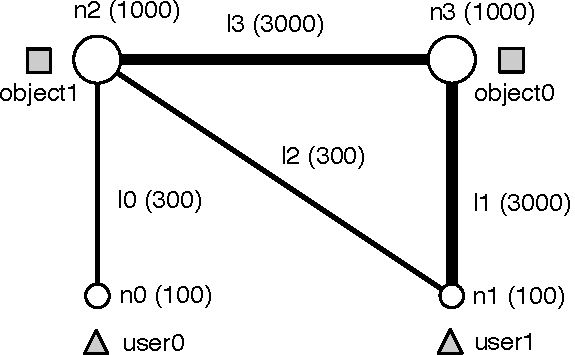
\includegraphics[width=7.5cm,clip]{topology-simple.pdf}
    \vspace{-2.0ex}
    \caption{simple simulation topology}
    \label{fig:topology-simple}
  \end{center}
\end{figure}

Simulation scenarios:
\begin{enumerate}
  \item	{\bf node only:} 4 nodes without randomization to show how the
        cost function works
  \item	{\bf link only:} 4 links without randomization to show
        different costs affects
  \item	{\bf monotonic function:} same as above but use monotonic cost
        function.
  \item	{\bf randomize:} 4 nodes and 4 links with randomization
  \item {\bf comparison:} compared with, no idle-resource pooling
  \item	{\bf surge:} same as above but with a request surge at one location
  \item	{\bf edge computing:} 2 nodes (big and small) and 1 link, the
    users are closer to the small node. 2 types jobs (interactive,
    data intensive).  show interactive jobs are on the small node,
    data intensive jobs are on the big node.
  \item {\bf premium service:} 4 nodes with 3 standard and 1 premium services.
  \item	{\bf complex?:} realistic scenario
\end{enumerate}
